
%% bare_conf.tex
%% V1.4a
%% 2014/09/17
%% by Michael Shell
%% See:
%% http://www.michaelshell.org/
%% for current contact information.
%%
%% This is a skeleton file demonstrating the use of IEEEtran.cls
%% (requires IEEEtran.cls version 1.8a or later) with an IEEE
%% conference paper.
%%
%% Support sites:
%% http://www.michaelshell.org/tex/ieeetran/
%% http://www.ctan.org/tex-archive/macros/latex/contrib/IEEEtran/
%% and
%% http://www.ieee.org/

%%*************************************************************************
%% Legal Notice:
%% This code is offered as-is without any warranty either expressed or
%% implied; without even the implied warranty of MERCHANTABILITY or
%% FITNESS FOR A PARTICULAR PURPOSE! 
%% User assumes all risk.
%% In no event shall IEEE or any contributor to this code be liable for
%% any damages or losses, including, but not limited to, incidental,
%% consequential, or any other damages, resulting from the use or misuse
%% of any information contained here.
%%
%% All comments are the opinions of their respective authors and are not
%% necessarily endorsed by the IEEE.
%%
%% This work is distributed under the LaTeX Project Public License (LPPL)
%% ( http://www.latex-project.org/ ) version 1.3, and may be freely used,
%% distributed and modified. A copy of the LPPL, version 1.3, is included
%% in the base LaTeX documentation of all distributions of LaTeX released
%% 2003/12/01 or later.
%% Retain all contribution notices and credits.
%% ** Modified files should be clearly indicated as such, including  **
%% ** renaming them and changing author support contact information. **
%%
%% File list of work: IEEEtran.cls, IEEEtran_HOWTO.pdf, bare_adv.tex,
%%                    bare_conf.tex, bare_jrnl.tex, bare_conf_compsoc.tex,
%%                    bare_jrnl_compsoc.tex, bare_jrnl_transmag.tex
%%*************************************************************************


% *** Authors should verify (and, if needed, correct) their LaTeX system  ***
% *** with the testflow diagnostic prior to trusting their LaTeX platform ***
% *** with production work. IEEE's font choices and paper sizes can       ***
% *** trigger bugs that do not appear when using other class files.       ***                          ***
% The testflow support page is at:
% http://www.michaelshell.org/tex/testflow/



\documentclass[conference]{IEEEtran}
% Some Computer Society conferences also require the compsoc mode option,
% but others use the standard conference format.
%
% If IEEEtran.cls has not been installed into the LaTeX system files,
% manually specify the path to it like:
% \documentclass[conference]{../sty/IEEEtran}





% Some very useful LaTeX packages include:
% (uncomment the ones you want to load)


% *** MISC UTILITY PACKAGES ***
%
%\usepackage{ifpdf}
% Heiko Oberdiek's ifpdf.sty is very useful if you need conditional
% compilation based on whether the output is pdf or dvi.
% usage:
% \ifpdf
%   % pdf code
% \else
%   % dvi code
% \fi
% The latest version of ifpdf.sty can be obtained from:
% http://www.ctan.org/tex-archive/macros/latex/contrib/oberdiek/
% Also, note that IEEEtran.cls V1.7 and later provides a builtin
% \ifCLASSINFOpdf conditional that works the same way.
% When switching from latex to pdflatex and vice-versa, the compiler may
% have to be run twice to clear warning/error messages.






% *** CITATION PACKAGES ***
%
%\usepackage{cite}
% cite.sty was written by Donald Arseneau
% V1.6 and later of IEEEtran pre-defines the format of the cite.sty package
% \cite{} output to follow that of IEEE. Loading the cite package will
% result in citation numbers being automatically sorted and properly
% "compressed/ranged". e.g., [1], [9], [2], [7], [5], [6] without using
% cite.sty will become [1], [2], [5]--[7], [9] using cite.sty. cite.sty's
% \cite will automatically add leading space, if needed. Use cite.sty's
% noadjust option (cite.sty V3.8 and later) if you want to turn this off
% such as if a citation ever needs to be enclosed in parenthesis.
% cite.sty is already installed on most LaTeX systems. Be sure and use
% version 5.0 (2009-03-20) and later if using hyperref.sty.
% The latest version can be obtained at:
% http://www.ctan.org/tex-archive/macros/latex/contrib/cite/
% The documentation is contained in the cite.sty file itself.






% *** GRAPHICS RELATED PACKAGES ***
%
\ifCLASSINFOpdf
  % \usepackage[pdftex]{graphicx}
  % declare the path(s) where your graphic files are
  % \graphicspath{{../pdf/}{../jpeg/}}
  % and their extensions so you won't have to specify these with
  % every instance of \includegraphics
  % \DeclareGraphicsExtensions{.pdf,.jpeg,.png}
\else
  % or other class option (dvipsone, dvipdf, if not using dvips). graphicx
  % will default to the driver specified in the system graphics.cfg if no
  % driver is specified.
  % \usepackage[dvips]{graphicx}
  % declare the path(s) where your graphic files are
  % \graphicspath{{../eps/}}
  % and their extensions so you won't have to specify these with
  % every instance of \includegraphics
  % \DeclareGraphicsExtensions{.eps}
\fi
% graphicx was written by David Carlisle and Sebastian Rahtz. It is
% required if you want graphics, photos, etc. graphicx.sty is already
% installed on most LaTeX systems. The latest version and documentation
% can be obtained at: 
% http://www.ctan.org/tex-archive/macros/latex/required/graphics/
% Another good source of documentation is "Using Imported Graphics in
% LaTeX2e" by Keith Reckdahl which can be found at:
% http://www.ctan.org/tex-archive/info/epslatex/
%
% latex, and pdflatex in dvi mode, support graphics in encapsulated
% postscript (.eps) format. pdflatex in pdf mode supports graphics
% in .pdf, .jpeg, .png and .mps (metapost) formats. Users should ensure
% that all non-photo figures use a vector format (.eps, .pdf, .mps) and
% not a bitmapped formats (.jpeg, .png). IEEE frowns on bitmapped formats
% which can result in "jaggedy"/blurry rendering of lines and letters as
% well as large increases in file sizes.
%
% You can find documentation about the pdfTeX application at:
% http://www.tug.org/applications/pdftex





% *** MATH PACKAGES ***
%
%\usepackage[cmex10]{amsmath}
% A popular package from the American Mathematical Society that provides
% many useful and powerful commands for dealing with mathematics. If using
% it, be sure to load this package with the cmex10 option to ensure that
% only type 1 fonts will utilized at all point sizes. Without this option,
% it is possible that some math symbols, particularly those within
% footnotes, will be rendered in bitmap form which will result in a
% document that can not be IEEE Xplore compliant!
%
% Also, note that the amsmath package sets \interdisplaylinepenalty to 10000
% thus preventing page breaks from occurring within multiline equations. Use:
%\interdisplaylinepenalty=2500
% after loading amsmath to restore such page breaks as IEEEtran.cls normally
% does. amsmath.sty is already installed on most LaTeX systems. The latest
% version and documentation can be obtained at:
% http://www.ctan.org/tex-archive/macros/latex/required/amslatex/math/





% *** SPECIALIZED LIST PACKAGES ***
%
%\usepackage{algorithmic}
% algorithmic.sty was written by Peter Williams and Rogerio Brito.
% This package provides an algorithmic environment fo describing algorithms.
% You can use the algorithmic environment in-text or within a figure
% environment to provide for a floating algorithm. Do NOT use the algorithm
% floating environment provided by algorithm.sty (by the same authors) or
% algorithm2e.sty (by Christophe Fiorio) as IEEE does not use dedicated
% algorithm float types and packages that provide these will not provide
% correct IEEE style captions. The latest version and documentation of
% algorithmic.sty can be obtained at:
% http://www.ctan.org/tex-archive/macros/latex/contrib/algorithms/
% There is also a support site at:
% http://algorithms.berlios.de/index.html
% Also of interest may be the (relatively newer and more customizable)
% algorithmicx.sty package by Szasz Janos:
% http://www.ctan.org/tex-archive/macros/latex/contrib/algorithmicx/




% *** ALIGNMENT PACKAGES ***
%
%\usepackage{array}
% Frank Mittelbach's and David Carlisle's array.sty patches and improves
% the standard LaTeX2e array and tabular environments to provide better
% appearance and additional user controls. As the default LaTeX2e table
% generation code is lacking to the point of almost being broken with
% respect to the quality of the end results, all users are strongly
% advised to use an enhanced (at the very least that provided by array.sty)
% set of table tools. array.sty is already installed on most systems. The
% latest version and documentation can be obtained at:
% http://www.ctan.org/tex-archive/macros/latex/required/tools/


% IEEEtran contains the IEEEeqnarray family of commands that can be used to
% generate multiline equations as well as matrices, tables, etc., of high
% quality.




% *** SUBFIGURE PACKAGES ***
%\ifCLASSOPTIONcompsoc
%  \usepackage[caption=false,font=normalsize,labelfont=sf,textfont=sf]{subfig}
%\else
%  \usepackage[caption=false,font=footnotesize]{subfig}
%\fi
% subfig.sty, written by Steven Douglas Cochran, is the modern replacement
% for subfigure.sty, the latter of which is no longer maintained and is
% incompatible with some LaTeX packages including fixltx2e. However,
% subfig.sty requires and automatically loads Axel Sommerfeldt's caption.sty
% which will override IEEEtran.cls' handling of captions and this will result
% in non-IEEE style figure/table captions. To prevent this problem, be sure
% and invoke subfig.sty's "caption=false" package option (available since
% subfig.sty version 1.3, 2005/06/28) as this is will preserve IEEEtran.cls
% handling of captions.
% Note that the Computer Society format requires a larger sans serif font
% than the serif footnote size font used in traditional IEEE formatting
% and thus the need to invoke different subfig.sty package options depending
% on whether compsoc mode has been enabled.
%
% The latest version and documentation of subfig.sty can be obtained at:
% http://www.ctan.org/tex-archive/macros/latex/contrib/subfig/




% *** FLOAT PACKAGES ***
%
%\usepackage{fixltx2e}
% fixltx2e, the successor to the earlier fix2col.sty, was written by
% Frank Mittelbach and David Carlisle. This package corrects a few problems
% in the LaTeX2e kernel, the most notable of which is that in current
% LaTeX2e releases, the ordering of single and double column floats is not
% guaranteed to be preserved. Thus, an unpatched LaTeX2e can allow a
% single column figure to be placed prior to an earlier double column
% figure. The latest version and documentation can be found at:
% http://www.ctan.org/tex-archive/macros/latex/base/


%\usepackage{stfloats}
% stfloats.sty was written by Sigitas Tolusis. This package gives LaTeX2e
% the ability to do double column floats at the bottom of the page as well
% as the top. (e.g., "\begin{figure*}[!b]" is not normally possible in
% LaTeX2e). It also provides a command:
%\fnbelowfloat
% to enable the placement of footnotes below bottom floats (the standard
% LaTeX2e kernel puts them above bottom floats). This is an invasive package
% which rewrites many portions of the LaTeX2e float routines. It may not work
% with other packages that modify the LaTeX2e float routines. The latest
% version and documentation can be obtained at:
% http://www.ctan.org/tex-archive/macros/latex/contrib/sttools/
% Do not use the stfloats baselinefloat ability as IEEE does not allow
% \baselineskip to stretch. Authors submitting work to the IEEE should note
% that IEEE rarely uses double column equations and that authors should try
% to avoid such use. Do not be tempted to use the cuted.sty or midfloat.sty
% packages (also by Sigitas Tolusis) as IEEE does not format its papers in
% such ways.
% Do not attempt to use stfloats with fixltx2e as they are incompatible.
% Instead, use Morten Hogholm'a dblfloatfix which combines the features
% of both fixltx2e and stfloats:
%
% \usepackage{dblfloatfix}
% The latest version can be found at:
% http://www.ctan.org/tex-archive/macros/latex/contrib/dblfloatfix/




% *** PDF, URL AND HYPERLINK PACKAGES ***
%
%\usepackage{url}
% url.sty was written by Donald Arseneau. It provides better support for
% handling and breaking URLs. url.sty is already installed on most LaTeX
% systems. The latest version and documentation can be obtained at:
% http://www.ctan.org/tex-archive/macros/latex/contrib/url/
% Basically, \url{my_url_here}.




% *** Do not adjust lengths that control margins, column widths, etc. ***
% *** Do not use packages that alter fonts (such as pslatex).         ***
% There should be no need to do such things with IEEEtran.cls V1.6 and later.
% (Unless specifically asked to do so by the journal or conference you plan
% to submit to, of course. )


% correct bad hyphenation here
\hyphenation{op-tical net-works semi-conduc-tor}

\usepackage[brazilian]{babel}   
\usepackage[utf8]{inputenc} 
\usepackage[pdftex]{graphicx}
\usepackage[version=3]{mhchem}
\usepackage{caption}
\usepackage{chemfig}
\usepackage{enumerate}
\usepackage{multirow}

\DeclareCaptionLabelFormat{lc}{\MakeLowercase{#1}~#2}
\captionsetup{labelfont=sc,labelformat=lc}

%Algoritmo
\usepackage[portuguese,ruled,lined,linesnumbered]{algorithm2e}




\begin{document}
	
\title{Multi objective evolutionary algorithms applied to protein structure prediction problem}

\author{Vidal Daniel da Fontoura, Ricardo Remes de Lima, Aurora Trinidad Ramirez Pozo e Roberto Santana Hermida}



% make the title area
\maketitle

% As a general rule, do not put math, special symbols or citations
% in the abstract
\begin{abstract}
%\boldmath
Many heuristics methods have been applied with
success to the PSP using simplified models for representation of
the problem. This methods usually minimize the free energy of a
protein structure. This study aimed the application of multiobjective
genetic algorithms combined with a relative representation
for the 2D-HP prediction model. Experiments were conducted
with two well-known algorithms: Non-dominated sorting Genetic
Algorithm II (NSGAII) and Indicator-Based Evolutionary Algorithm
(IBEA). Moreover, the algorithms are evaluated and compared using different
genetic operators.

\end{abstract}

% no keywords




% For peer review papers, you can put extra information on the cover
% page as needed:
% \ifCLASSOPTIONpeerreview
% \begin{center} \bfseries EDICS Category: 3-BBND \end{center}
% \fi
%
% For peerreview papers, this IEEEtran command inserts a page break and
% creates the second title. It will be ignored for other modes.
\IEEEpeerreviewmaketitle



\section{Introdução}

The proteins play a fundamental role in the nature. These structures, made of aminoacids, participate in many of the most important tasks of the living cells. Proteins guarantee the correct functioning of a large number of biological function in nature. The protein structure is the result of the so-called protein folding process in which the initially unfolded chain of aminoacids is transformed into its final structure. Under suitable
conditions, this structure is uniquely determined by the sequence. COLOCAR REFERNCIA ROBERTO.



Uma proteína é uma macromolécula composta por uma sequência de aminoácidos. Sua  função biológica é determinada pelo molde de sua estrutura. Entender como as proteínas se moldam é de grande importância para a biologia, bioquímica e medicina. Entretanto não é possível determinar a estrutura exata de uma proteína utilizando o modelo atômico analítico completo, mesmo com os mais poderosos recursos computacionais \cite{lopes2008evolutionary}. 

Diante deste cenário, diferentes abordagens heurísticas vêm sendo desenvolvidas para reduzir a complexidade computacional envolvida na determinação da estrutura de proteínas. Dentre elas, existem estudos que exploram a predição de estrutura de proteínas 
combinadas com algoritmos evolutivos como, por exemplo, Li et al. \cite{li2012genetic} que propõem um AE (Algoritmo Evolucionário) mono-objetivo em conjunto com uma estratégia de busca local para o problema PSP utilizando o modelo simplificado Hidrofóbico-Polar (HP). Já Soares et al. \cite{soares2011investigating} propõem um algoritmo multiobjetivo em tabelas e comparam seu desempenho em relação ao NSGAII \cite{deb2002fast}, otimizando duas funções de energia de grande importância no processo de conformação: van der Waals e eletroestática. Gabriel et al. \cite{gabriel2012algoritmos} também propõem a utilização de um algoritmo multiobjetivo em tabelas similar ao proposto em \cite{soares2011investigating}, porém utilizando o modelo HP para representação e avaliação das soluções.

Este trabalho propõem a aplicação e comparação dos algoritmos genéticos multiobjetivo NSGAII e IBEA \cite{zitzler2004indicator} com o primeiro objetivo de minimizar a energia calculada a partir do modelo HP e um segundo objetivo que busca minimizar a distância euclidiana entre aminoácidos de uma proteína.

O artigo está organizado da seguinte maneira: na seção II é apresentado o problema PSP, modelo
HP, e a representação relativa para o modelo HP. A seção III discorre sobre algoritmos genéticos e otimização multiobjetivo. A seção IV apresenta os métodos comparados. A seção V explica os experimentos que foram conduzidos. A seção VI apresenta os trabalhos correlatos. Por fim a seção VII conclui a análise sobre os experimentos e menciona os possíveis incrementos a este estudo.


\section{Problema de Predição de estruturas de Proteínas}
O problema PSP trata da determinação da estrutura final de uma proteína utilizando apenas informação referente a sua sequencia de aminoácidos \cite{dorn2014three}. Uma abordagem computacional para predizer a estrutura de uma proteína necessita de um modelo que a represente de maneira abstrata num certo nível de detalhamento. Baseada nas leis da termodinâmica a predição é modelada a partir da minimização da energia livre correspondente às possíveis conformações que uma proteína pode obter. Formalmente a conformação nativa de uma proteína é definida como a conformação em que a energia livre é mínima. O nível de detalhamento dos modelos pode variar. Por exemplo, a estrutura da proteína poderia ser representada apenas pelos átomos que compõem o \textit{backbone} desconsiderando ramificações laterais, por uma representação espacial de todos os seus átomos, por todos os átomos exceto o hidrogênio ou apenas os elementos hidrofóbicos-polares representados em rede\cite{lopes2008evolutionary}.


\subsection{Modelo HP}
O modelo Hidrofóbico-Polar, ou modelo HP, desenvolvido por Lau e Dill  \cite{lau1989lattice}, é um modelo em rede, dentre outros, que é utilizado nas pesquisas para PSP, e, assim como os demais, é um modelo de representação de proteínas que possui simplificações. O modelo considera apenas dois tipos de resíduos: o Hidrofóbico (H) e o Hidrofílico ou Polar (P). Uma proteína é constituída por uma sequência destes resíduos posicionados em uma grade (do inglês \textit{lattice}) regular, de forma a construir um caminho que não se cruza \cite{santana2008protein}. Neste modelo, o principal conceito utilizado é o conceito de vizinhança. Dados dois resíduos, eles são considerados vizinhos caso sejam adjacentes na grade e na sequência (vizinhos ligados) ou apenas adjacentes na grade (vizinhos topológicos). A Figura \ref{fig1} apresenta um exemplo de uma sequência no modelo HP, onde os círculos pretos representam os resíduos H e, os brancos resíduos P. Vizinhos ligados estão representados pela linha contínua, enquanto que vizinhos topológicos estão circulados com uma elipse tracejada.

\begin{figure}[ht]
	\centering
	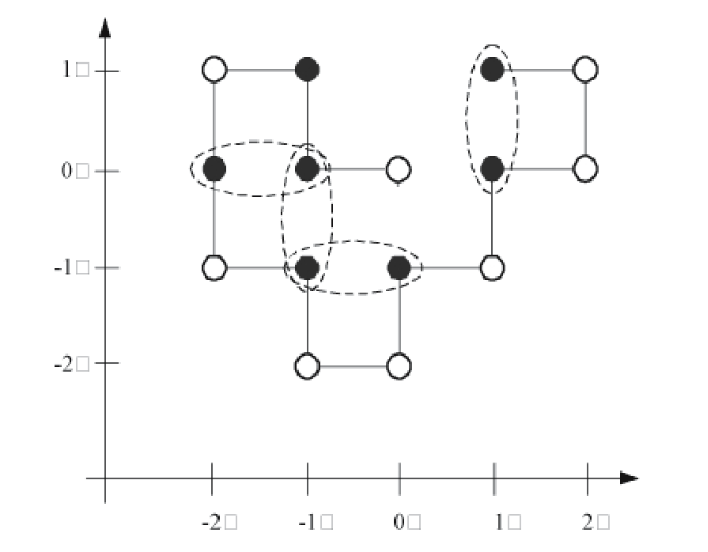
\includegraphics[width=2.5in]{figure1.png}
	\caption{Conformação hipotética de uma cadeia de 15 aminoacídos utilizando modelo 2D-HP. Adaptado de \cite{lopes2008evolutionary}}.
	\label{fig1}
\end{figure}

No modelo HP, dependendo do par de resíduos que formam um contato topológico (vizinhos topológicos), são atribuídos os seguintes valores: HH=-1 e HP = PP = 0. A energia livre de uma conformação é inversamente proporcional ao número de vizinhos topológicos HH. Consequentemente, minimizar a energia livre é equivalente a maximizar a quantidade de vizinhos topológicos onde o par é composto por resíduos hidrofóbicos (HH) \cite{lopes2008evolutionary}.


\subsection{Representação relativa}

A representação relativa para o modelo HP se baseia na construção da estrutura da proteína utilizando uma sequência de direções. Nesta abordagem, cada resíduo tem sua posição definida relativamente ao resíduo anterior \cite{lopes2008evolutionary}. Para uma cadeia de N resíduos, a partir do primeiro que é fixo, todo resíduo subsequente é posicionado de acordo com uma dada direção. Para o modelo 2D-HP apenas três direções são possíveis:

\begin{itemize}
	\item Em frente: continuar na mesma direção em que estava;
	\item Virar à direita: posicionar o resíduo à direita do anterior;
	\item Virar à esquerda: posicionar o resíduo à esquerda do anterior.
\end{itemize}


A cada resíduo que é colocado, a direção atual é atualizada. Desta forma, os comandos “seguir em frente”, “virar à direita” e “virar à esquerda” vão estar todos baseados no resíduo anterior, como mostra a figura \ref{fig2}. 

\begin{figure}[ht]
	\centering
	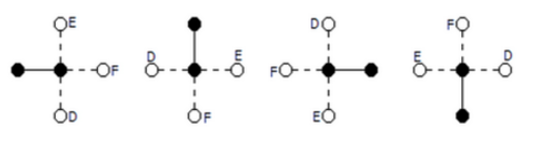
\includegraphics[width=2.5in]{figure2.png}
	\caption{Representação relativa, onde F significa um movimento em frente, D movimento a direita e E um movimento a esquerda.}
	\label{fig2}
\end{figure}


\section{Algoritmos Evolucionários e Otimização Multiobjetiva}
Algoritmos Evolucionários (EAs - Evolutionary Algorithms) são uma técnica de busca e otimização, altamente paralela, inspirada no princípio Darwiniano de seleção natural e reprodução genética. Os princípios da natureza nos quais os EAs se inspiram são simples. De acordo com a teoria de C. Darwin, o princípio de seleção privilegia os indivíduos com maior aptidão, portanto, com maior probabilidade de reprodução. Indivíduos com mais descendentes têm mais chance de perpetuarem seus códigos genéticos nas próximas gerações. Tais códigos genéticos constituem a identidade de cada indivíduo e estão representados nos cromossomos. Estes princípios são imitados na construção de algoritmos computacionais, que buscam uma melhor solução para um determinado problema através da evolução de populações de soluções codificadas por cromossomos artificiais – estrutura de dados utilizada para representar uma possível solução para o problema na execução do algoritmo \cite{pacheco1999algoritmos}. 
Problemas do mundo real costumam ter múltiplos objetivos a serem minimizados/maximizados e estão presentes na maioria das áreas do conhecimento. Para otimizar problemas multiobjetivos são considerados 2 ou mais objetivos que costumam ser conflitantes entre si. Para estes problemas não é possível encontrar uma única solução. Um conjunto de soluções ótimas é alcançado avaliando a relação de dominância de Pareto \cite{pareto} entre as soluções. O objetivo é encontrar as soluções que não são dominadas por nenhuma outra. Uma solução domina outra, se e somente se, for melhor em pelo menos um dos objetivos, sem ser pior em nenhum dos outros objetivos. O conjunto de soluções não dominadas formam a fronteira de Pareto. Encontrar a fronteira de Pareto real é NP-Difícil \cite{fonseca2005tutorial}, portanto o objetivo é encontrar uma boa aproximação desta fronteira.
MOEAs (Multi-Objective Evolutionary Algorithms) são extensões de AEs para problemas multiobjetivos que aplicam os  conceitos de dominância de Pareto para criar estratégias distintas para evoluir e diversificar as soluções. Neste trabalho foram utilizados dois MOEAs: NSGAII \cite{deb2002fast} e IBEA \cite{zitzler2004indicator}.

\subsection{NSGAII (Non-dominated sorting Genetic Algorithm II)}
Este algoritmo tem como principal característica um forte mecanismo de elitismo, classificando, a cada geração, todas as soluções em diferentes \textit{fronts} de acordo com a relação de não-dominância (linha 15 do Algoritmo 1). Após a classificação, soluções pertecentes ao primeiro \textit{front}, são não dominadas por nenhuma outra solução, soluções pertecentes ao segundo \textit{front} são dominadas apenas pelas soluções contidas no primeiro \textit{front}, da mesma maneira soluções do terceiro \textit{front} são dominadas por soluções do segundo e do primeiro \textit{front} e assim por diante. Para soluções de uma mesma \textit{front} o NSGAII utiliza o operador de \textit{crowding distance}, para calcular o quão distante estão os vizinhos de uma determinada solução (linha 19 do Algoritmo 1). Soluções com o valor de \textit{crowding distance} maior são priorizados pois irão contribuir com uma maior diversidade para a população (linha 23 e 24 do Algoritmo 1). Ambas classificações são utilizadas pelo operador de seleção (linha 24 do Algoritmo 1). O torneio binário seleciona soluções do menor \textit{front} e com maiores valores de \textit{crowding distance}. Uma nova população é gerada utilizando os operadores de cruzamento e mutação (linha 25 do Algoritmo 1).


\begin{algorithm}[ht]
	\Entrada{\\N // Tamanho da População \\T // Quantidade máxima de avaliações}
	
	\Saida{\\P // Conjunto de soluções não dominadas}
	\Inicio{
		$P_0 \gets Inicilizar\_Populacao(n);$\\
		$AtribuicaoFitness(P_0);$\\
		$FastNonDominatedSort(P_0);$\\
		$Q_0 \gets 0;$\\
		\Enqto{$Q_0 < N$}{
			$Parents \gets TorneioBinario(P_0);$\\
			$Children \gets CruzamentoMutacao(Parents);$\\
			$Q_0 \gets Children;$\\
		}
		$AtribuicaoFitness(Q_0);$\\
		
		$t \gets 0;$\\
		\Enqto{$t < T$} {	
			$R_t \gets P_t \cup Q_t;$\\
			$Fronts \gets FastNonDominatedSort(R_t);$\\
			$P_{t+1} \gets 0;$\\
			$i \gets 0;$\\
			
			\Enqto{$P_{t+1} + Front_i  < N$} {
				$CrowdingDistanceAssignment(Front_i);$\\
				$P_{t+1} \gets P_{t+1} \cup Front_i;$\\
				$i \gets i + 1;$\\
			}
			$CrowdingDistanceSort(Front_i)$;
			$P_{t+1} \gets P_{t+1} \cup Front_i[1:(N -P_{t+1} )]$ //Preenche 	$P_{t+1}$ com as melhores soluções da //$Front_i$ segundo o critério de \textit{crowding-distance}  \\
			
			$Parents \gets TorneioBinario(P_{t+1})$;\\
			$Q_{t+1} \gets CruzamentoMutacao(Parents)$;
			
			$t \gets t +1$;
		}
	}
	\caption{NSGAII}
\end{algorithm}


\subsection{IBEA (Indicator-Based Evolutionary Algorithm)}
No contexto de otimização multiobjetiva, otimizar consiste em encontrar uma fronteira ótima com uma boa aproximação da fronteira de Pareto. Contudo não existe uma definição geral do que é uma boa aproximação. Dessa forma, indicadores costumam ser utilizados para avaliar a qualidade de uma fronteira aproximada. O \footnotemark{\textit{hypervolume}} é um exemplo de indicador para avaliação e comparação de fronteiras. 
O IBEA é um algoritmo que considera
a otimização de indicadores de qualidade. O indicador é a maneira de avaliar o conjunto não dominado de soluções \cite{figueiredo2013algoritmo}.
Para utilizar o IBEA é necessário definir o indicador que será utilizado para associar cada par ordenado de soluções a um valor escalar. Um dos indicadores mais utilizados é o \textit{hypervolume} devido a sua capacidade de avaliar a convergência e diversidade ao mesmo tempo no processo de busca \cite{ishibuchi2008evolutionary}. 

Dada uma população $P$ que representa uma amostra do espaço de busca e um indicador $I$, a aptidão (\textit{fitness}) de uma solução é dada de acordo com a sua contribuição, em relação aos objetivos, ao processo de otimização (linha 3 do algoritmo 2). A função de aptidão $F$ utilizada pelo IBEA é definida pela equação \ref{calcFitnessIBEA}.

\begin{equation}
\ F(x_i) = \sum_{x_j \in (P-x_i)} {-e^\frac{-I_{Hy}(x_j,x_i)}{k}}
\label{calcFitnessIBEA}
\end{equation}
%\begin{equation}

%	$F(x_i)= \sum_{x_j \in %(P-x_i)}{-e^\frac{-I_{HD}(x_j,x_i)}{k}}$

%\end{equation}

onde $k$ é um parâmetro normalmente ajustado para 0,05. O valor $F(x_i)$ corresponde a uma medida da perda de qualidade da aproximação da fronteira de Pareto se a solução $x_i$ for removida da população \cite{figueiredo2013algoritmo} baseado no valor do indicador qualidade $I_{Hy}$, neste caso 
\textit{hypervolume}.
Baseado no cálculo de \textit{fitness} descrito acima o algoritmo básico do IBEA consiste em realizar de forma iterativa a seleção (linha 10 do algoritmo 2), cruzamento, mutação (linha 11 do algoritmo 2) e seleção ambiental, removendo o pior indivíduo da população e atualizando os valores de aptidão dos indivíduos restantes (linhas 4 a 8 do algoritmo 2).

%	{\LinesNumberedHidden
\begin{algorithm}[h]
	
	\Entrada{\\N // Tamanho da População \\T // Quantidade maxima de avaliações\\ k //Fator de escalonamento do fitness}
	
	\Saida{\\P // Conjunto de soluções não dominadas}
	Criação de uma população inicial $P$ de tamanho $N$\\
	Inicializa o contador $m \gets 0$\\
	Atribui valor \textit{fitness} do indivíduos contidos em $P$ utilizando a equação descrita na \ref{calcFitnessIBEA}\\ 	
	
	%Executa os 3 passos a seguir até que o tamanho da população $P$ não exceda $N$:\\
	\Enqto{$P > N$} { 
		Seleciona o indivíduo $x^*$ com o menor valor de \textit{fitness}\\
		Remover $x^*$ da população $P$\\
		Atualizar os valores de \textit{fitness} dos indivíduos restantes utilizando a equação apresentada na figura 3, sendo $x_j$ igual a $x^*$, para todo $x \in P$.\\
	}
	
	
	Se $m >= T$ ou outro critério de parada for alcançado $A \gets P$. Execução termina e $A$ é retornado. \\
	
	Seleciona indivíduos via torneio binário  com troca da população $P$ para gerar uma população temporária $\overline P$\\
	
	Os operadores de cruzamento e mutação  são aplicados em $\overline P$ e adicionado os descendentes resultantes em $P$. Incrementa $(m = m+1)$ e a execução retorna a linha 3.
	\caption{IBEA}
\end{algorithm}%}

\footnotetext[1]{\textit{Hypervolume} : Indicador de qualidade proposto e utilizado inicialmente no estudo \cite{zitzler1998multiobjective}, denotado como o "tamanho do espaço de busca coberto". Este indicador tem duas vantagens importantes em relação a outros indicadores: \cite{zitzler2007hypervolume} 1 - Sensitivo a qualquer tipo de melhoria de conjunto de aproximação em relação a outro conjunto. 2 - Como resultado de 1, o indicador garante que para qualquer conjunto de aproximação \textit{A} que obtenha os maiores valores de \text{hypervolume} contém todas as soluções da fronteira ótima de Pareto.} 

\section{Métodos Comparados}

The algorithms NSGAII and IBEA were applied to the PSP problem with the relative representation to 2D-HP model. The multi objective optimization framework jMetal \cite{jMetal} it was used since it contains the implementation of both MOEAs. In order to evaluate the solutions found by the algorithms, a mechanism which considers two objectives was implemented. Next both objectives are listed: 

O método proposto consistiu na aplicação dos algoritmos NSGAII e IBEA ao problema PSP utilizando a representação relativa aplicada o modelo HP. O framework de otimização multiobjetiva jMetal \cite{jMetal} foi utilizado pois contém implementações para MOEAs utilizados. Para avaliar as soluções geradas pelos algoritmos, um mecanismo de avaliação foi implementado levando em consideração dois objetivos:

\begin{enumerate}[I]
	\item{Maximizar a quantidade de vizinhos topológicos HH (objetivo principal)}
	\item{Maximize the amount of topological contacts H-H (main objective)}
	\item{Minimizar a máxima distância euclidiana entre resíduos (objetivo secundário)}
		\item{Minimize the maximum eucledian distance between residues (secondary objective)}
\end{enumerate}

The first objective leads the search to regions of the search space where the minimum energy resides (by maximizing the amount of topological contacts H=H). In this manner, the goal is to obtain the closest structure  to the native conformation. The second objective allows to differentiate structures with the same energy value but with distinct levels of compactness. Usually structures with lower values of energy are more compact that the ones with higher values of energy. 

O primeiro objetivo guia a busca com intenção de encontrar a solução que gere uma estrutura onde o valor de energia seja mínimo (maximizando a quantidade de vizinhos topológicos HH), dessa maneira, obtendo uma estrutura mais próxima da conformação nativa de uma proteína. Já o segundo objetivo permite diferenciar soluções com o mesmo valor de energia mas com graus de compactação diferentes, pois quanto menor for o valor máximo para distancia euclidiana, mais compacta será a conformação gerada.

The chromosomes are represented by integer vectors where which gene specifies what direction, relative to the previous residue, must be placed the next residue. In the case of 2D-HP model: the genes can assume only three values (0,1,2) where 0 represents that next residue should be placed on the right of the previous one, 1 means that the next residue should be placed in front of the previous residue and 2 indicates that the next residue should be placed on the left of the previous residue. Figure \ref{fig_sim} shows a example of a hypothetical chromosome of a chain of 10 residues and the conformation generated by it.

Os cromossomos foram representados por vetores inteiros onde os genes especificam em qual direção, relativa ao resíduo anterior, deve ser posicionado o próximo resíduo. Os genes podem assumir um dos valores (0, 1, 2), onde 0 indica que o próximo resíduo deve ser posicionado a direita do resíduo anterior, 1 indica que o próximo resíduo deve ser posicionado a frente do resíduo anterior e 2 indica que o próximo resíduo deve ser posicionado a esquerda do resíduo anterior. A figura \ref{fig_sim} demonstra um exemplo de um possível cromossomo para uma cadeia de 10 resíduos e a conformação que é gerada por ele.

\begin{figure}[ht]
	\centering
	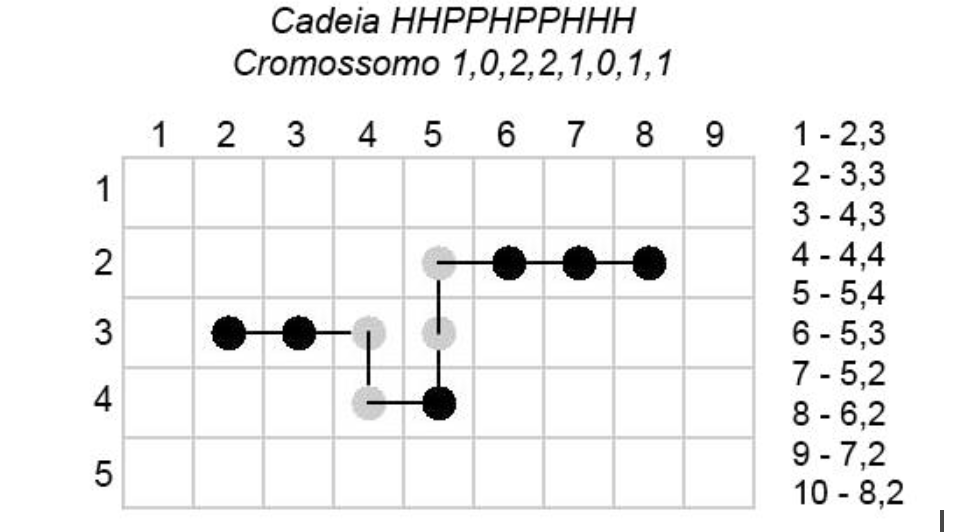
\includegraphics[width=2.5in]{figure3.png}
	\caption{Exemplo de conformação gerada a partir de um cromossomo utilizando a representação relativa.}
	\label{fig_sim}
\end{figure}

The relative representation of the 2D-HP model have a weak spot. Since the solutions are usually initiate randomly there is huge potential of generating many infeasible solutions. One solution is said to be infeasible when the generated structure is not self avoiding. In other words one solution is not feasible when a position of the grid is occupied by more than one residue. In order to avoid this problem a simple repair mechanism was designed. The algorithm 3 presents the pseudo-code of the repair mechanism.

A representação relativa está sujeita à geração de soluções infactíveis ao problema utilizando o modelo HP. Uma solução é considerada infactível quando um resíduo 'colide' com outro resíduo que já havia sido posicionado na grade. Um mecanismo de reparação simples foi desenvolvido a fim de contornar o problema de geração de soluções infactíveis e pode ser observado no algoritmo 3.

\begin{algorithm}[h]
	\label{algo:reparacao}
	Get the position that the next residue should be placed. \\
	Obtém a direção em que o próximo resíduo deve ser posicionado.\\
	Check if position is already occupied.\\
	Verifica se esta direção causará uma colisão.\\
	If the position is already occupied a new position is tried.\\
	Caso a colisão seja identificada uma nova direção é utilizada.\\
	Repeat the steps 2 e 3 until the residue be positioned. \\
	Repetir os passos 2,3 até que seja possível posicionar o próximo resíduo ou se todas as direções foram testadas e nenhuma não causa colisão.\\
	If the residue could be placed the repair mechanism has obtained success, otherwise ,the solution will be penalized further in the fitness evaluation.\\
	Se foi possível posicionar o próximo resíduo o mecanismo de reparação obteve sucesso, se por acaso não foi possível a solução é considerada infactível e será penalizada no processo de avaliação.
	\caption{Mecanismo de reparação de soluções infactíveis}
\end{algorithm}


This mechanism had to be designed because it was observed, in previous experiments, that a substantial number of infeasible solutions were present in the initial population. It is worthwhile to mention that the repair mechanism can not ensure that all solutions, from the initial population, are feasible and they are penalized subtracting the amount of collisions from the amount of topological contacts H-H. 

Este mecanismo foi implementado pois foi observado em experimentos prévios que o numero de soluções infactíveis era muito grande. É necessário mencionar que mesmo utilizando o mecanismo de reparação soluções infactíveis ainda podem ser geradas pois o mecanismo nem sempre consegue reparar. Contudo soluções infactíveis são penalizadas subtraindo a quantidade de colisões da quantidade de vizinhos topológicos HH.

Usually indicators of quality are used to evaluate and compare the performance of MOEA's. In this study it was utilized the hypervolume indicator. This indicator considers the area of the search space that a given front dominates it. The larger the hypevolume value, better the quality of the optimum front found by a given MOEA.


Para  avaliar e comparar o desempenho dos algoritmos multiobjetivos, indicadores de qualidade costumam ser utilizados. Neste estudo foi utilizado o indicador \textit{hypervolume}, o qual considera o volume do espaço de busca dominado por uma fronteira ótima\cite{zitzler2003performance}. Quanto maior o \textit{hypervolume} melhor é qualidade da fronteira ótima encontrada por um algoritmo.

\section{Experimentos e Resultados}

Experiments were conducted using the algorithms NSGAII and IBEA described na seção IV. A set of parameters configuration were used in order to find the best configuration for each algorithm. For the IBEA algorithm a total of 120 distinct configurations were used.
Experimentos foram conduzidos utilizando os algoritmos NSGAII e IBEA apresentados na seção IV. Uma variação e combinação de parâmetros foi realizada para encontrar a melhor configuração de cada algoritmo. Resultando em 120 configurações para o algoritmo IBEA e 60 para o algortimo NSGAII visto que este não utiliza população auxiliar. A tabela \ref{tab:tuning} apresenta o  valores que foram variados nos experimentos.

\begin{table}[h]
	\centering
	\caption{Parâmetros utilizados nos experimentos}
	\label{tab:tuning}
	\begin{tabular}{|c|c|}
		\hline
		{\bf Parâmetro} & {\bf Valores}                 \\ \hline
		População       & 200,250,300,350,400           \\
		\hline
		Pop Aux. (IBEA)        & 200,300                       \\ \hline
		Avaliações      & 40000,60000,70000,100000      \\ \hline
		Cruzamento      & SinglePoint,TwoPoints,Uniform \\ \hline
		Taxa Cruz.      & 90\%                          \\ \hline
		Mutação         & BitFlip                       \\ \hline
		Taxa Mut.       & 0.01\%                        \\ \hline
	\end{tabular}
\end{table}

Para fins de comparação foi utilizada uma cadeia de 64 aminoácidos, a cadeia mais complexa utilizada no estudo desenvolvido por Li et al. (2012) \cite{li2012genetic}. A fórmula abaixo representa a sequência de aminoácidos:  
\\
\\
\begin{small}
	\noindent \ce{H12PHPHP2H2P2H2P2HP2H2P2H2P2HP2H2P2H2P2HPHPH12} 
\end{small}
\\

Por se tratarem de algoritmos estocásticos, cada configuração de algoritmo foi executado 30 vezes a fim de avaliar se o comportamento se mantém similar em todas as execuções, resultando em 30 fronteiras ótimas referentes a cada execução de cada algoritmo. 
Para cada fronteira foram removidas as soluções duplicadas e dominadas. As fronteiras resultantes foram submetidas à normalização, dessa maneira, harmonizando as escalas dos objetivos utilizados pelos algoritmos. O cálculo utilizado para normalização é apresentado na equação \ref{eq:calcNorma}.

\begin{equation}
\
Xnorm = X -MIN/ MAX -MIN\
\label{eq:calcNorma}
\end{equation}


Onde X deve assumir os valores encontrados para um dos objetivos e MIN e MAX são o menor e o maior valor encontrados para o objetivo em questão. 
A normalização é necessária pois os conjuntos de valores para cada objetivo tem escalas diferentes. Ao normalizar garantimos que ambos os valores encontrados para cada objetivo estarão na mesma escala, de 0 e 1 neste caso. Dessa maneira ao calcular os valores de \textit{hypervolume} evitamos que soluções com objetivos de escalas desproporcionais sejam priorizados.

Os valores de \textit{hypervolume} foram calculados para cada uma das fronteiras geradas a partir das 30 execuções de cada configuração. Os valores de média, desvio padrão, mínimo e máximo referente as 30 execuções foram calculados para cada configuração. A tabela \ref{tab:media} apresenta os valores de \textit{hypervolume}  da melhor configuração obtida para cada algoritmo e o resultado do teste estatístico Kruskal-Wallis \cite{kruskal1952use} entre as mesmas. Já a tabela \ref{tab:bestConfigs} apresenta a melhor configuração para cada algoritmo. 


\begin{table}[h]
	\centering
	\caption{Média, Desvio Padrão, Mínimo, Máximo e teste estatístico de Kruskal-Wallis}
	\label{tab:media}
	\scalebox{0.9}{
	\begin{tabular}{|c|c|c|c|c|c|}
		\hline
		Algoritmo & Média        & Desvio Padrão & Mínimo & Máximo & \multicolumn{1}{l|}{Kruskal-Wallis} \\ \hline
		NSGAII    & 0.5222       & 0.0429        & 0.4496 & 0.6025 & \multirow{2}{*}{TRUE}        \\ \cline{1-5}
		IBEA      & {\bf 0.5855} & 0.0711        & 0.4739 & 0.7799 &                              \\ \hline
	\end{tabular}}
	
\end{table}

É possível observar baseado nas médias de \textit{hypervolume}, com diferença estatística segundo o teste de Kruskal-Wallis, que o algoritmo IBEA obteve uma maior cobertura do espaço de busca quando comparado ao NSGAII. Dessa maneira podemos afirmar que o algoritmo IBEA obteve um desempenho melhor que o NSGAII pois a fronteira gerada pelo IBEA domina a fronteira gerada pelo NSGAII.


\begin{table}[h]
	\centering
	\caption{Melhores configurações de parâmetros para os algoritmos}
	\label{tab:bestConfigs}
	\scalebox{0.9}{
	\begin{tabular}{|c|c|c|p{0.4cm} |p{1.5cm}|p{1.3cm}|}
		\hline
		\textbf{Algoritmo} & 	\textbf{Avaliações} & 	\textbf{População} & 	\textbf{Pop Aux.} & 	\textbf{Cruzamento/\%}  & 	\textbf{Mutação/\% }    \\ \hline
		NSGAII    & 70000      & 350  & -    & TwoPoints/90\% & BitFlip/0.01\% \\ \hline
		IBEA      & 100000      & 400 & 200     & TwoPoints/90\% & BitFlip/0.01\% \\ \hline
	\end{tabular}}
\end{table}

Os melhores valores obtidos para o primeiro objetivo, de maximizar a quantidade de vizinhos topológicos, utilizando os algoritmos IBEA e NSGAII foram comparados com os resultados obtidos por métodos propostos em outros estudos que utilizaram a mesma sequência de aminoácidos, e são apresentados na tabela \ref{tab:comparacao}.

\begin{table}[h]
	\centering
	\caption{Comparação entre a quantidade de vizinhos topológicos obtidos pelos estudos.}
	\label{tab:comparacao}
	\begin{tabular}{|c|c|}
		\hline
		{\bf Metódo/Estudo} & {\bf Menor Valor de Energia} \\ \hline
		MC \cite{unger1993genetic}               & 35                          \\ \hline
		GA   \cite{unger1993genetic}               & 37                          \\ \hline
		SISPER  \cite{zhang2002new}            & 39                          \\ \hline
		ISA \cite{huang2005improved}                & 38                          \\ \hline
		GAOSS  \cite{huang2010protein}             & 42                          \\ \hline
		GA-pull-moves \cite{li2012genetic}      & 42                          \\ \hline
		IBEA                & 40          \\ \hline 
		NSGAII & 32 \\
		\hline
	\end{tabular}
\end{table}

Analisando apenas o objetivo de maximizar a quantidade de vizinhos topológicos observamos que o IBEA conseguiu encontrar uma solução com 40, ficando atrás apenas de duas abordagens propostas por: Li et al. (2012) \cite{li2012genetic} e Huang et al. (2010) \cite{huang2010protein}. Já o algoritmo NSGAII ficou atrás de todas as abordagens pois obteve um valor muito baixo de vizinhos HH.


As figuras \ref{bestSolutionIBEA} e \ref{bestSolutionNSGAII} apresentam respectivamente as soluções com a maior quantidade de vizinhos topológicos HH para o algoritmo IBEA e para o NSGAII.

\begin{figure}[ht]
	\centering
	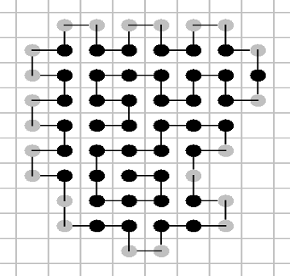
\includegraphics[width=1.5in]{ibeabestresults.png}
	\caption{Melhor solução obtida pelo algoritmo IBEA com 40 vizinhos topológicos HH.}
	\label{bestSolutionIBEA}
\end{figure}


\begin{figure}[ht]
	\centering
	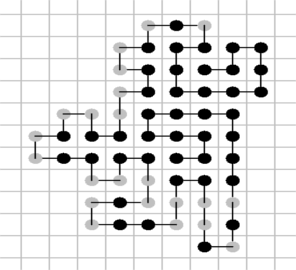
\includegraphics[width=1.5in]{nsgaiibestresults.png}
	\caption{Melhor solução obtida pelo algoritmo NSGAII com 32 vizinhos topológicos HH.}
	\label{bestSolutionNSGAII}
\end{figure}

\section{Trabalhos Correlatos}
Esta seção apresenta três trabalhos que possuem a
implementação de estratégias para algoritmos evolutivos
aplicados ao problema da PSP, e que serviram de base
para a proposta desenvolvida para este trabalho.

Li et al. (2012) \cite{li2012genetic} desenvolveram um AE mono-objetivo combinado a uma estratégia de busca local baseada em \textit{pull moves} para o modelo 2D-HP \cite{lesh2003complete}. Li et al. (2012) realizaram experimentos utilizando cadeias de 20 a 64 resíudos comparam os resultados obtidos com resultados de outros estudos e concluíram que abordagem proposta se mostrou eficiente quando comparada com outras estratégias utilizadas em estudos anteriores.

O estudo desenvolvido por Gabriel et al. (2012) \cite{gabriel2012algoritmos} propõe um algoritmo evolutivo multi-objetivo para o problema PSP utilizando o modelo HP, o qual avalia a
quantidade de contatos topológicos, assim como o grau de
compactação da conformação. Concluíram que sua abordagem
encontrou soluções com a mesma quantidade de contatos
hidrofóbicos que um algoritmo mono-objetivo, utilizando
populações menores do que as utilizadas em outras propostas
e demostrando um efeito positivo na utilização
de uma proposta multi-objetiva.

Já Soares et al. (2011) \cite{soares2011investigating} propuseram um AG multi-objetivo definindo o cálculo da energia de Van der Walls e o cálculo da energia eletroestática como os objetivos. Soares et al. (2011) realizaram experimentos com o algoritmo proposto e com o algoritmo NSGAII \cite{deb2002fast} e concluiram que o algoritmo proposto apresentou melhores resultados quando comparado ao NSGAII. 




\section{Conclusão e Trabalhos Futuros}

A partir dos experimentos realizados, foi possível constatar
que a aplicação de uma abordagem multiobjetiva para o problema PSP apresentou uma diferença entre os algoritmos IBEA e NSGAII. Verificamos uma diferença entre as médias de \textit{hypervolume} entre os algoritmos. Contudo apenas ao verificar a maior quantidade de vizinhos topológicos encontrados por cada algoritmo ficou nítida a diferença no desempenho dos algoritmos. Ao comparar o algoritmo IBEA com outros estudos que realizaram experimentos com a mesma sequência de aminoácidos observamos que de 7 estudos: 5 obtiveram valores inferiores ao obtido algoritmo IBEA e apenas 2 estudos obtiveram valores superiores. Por fim também concluímos que operador de cruzamento que apresentou melhor desempenho foi o \textit{TwoPoints} visto que foi aplicando este que os ambos os algoritmos NSGAII e IBEA obtiveram seus maiores resultados. 

Trabalhos futuros incluem a exploração de mais técnicas de cruzamento, mutação, seleção; utilização de hyperherísticas para seleção de operadores para os algoritmos; utilizar  outras sequências de aminoácidos;  introdução de outras técnicas de busca e adição de interface gráfica que viabilize interação entre usuários especialistas no domínio do problema com os MOEAs. 
% conference papers do not normally have an appendix





% trigger a \newpage just before the given reference
% number - used to balance the columns on the last page
% adjust value as needed - may need to be readjusted if
% the document is modified later
%\IEEEtriggeratref{8}
% The "triggered" command can be changed if desired:
%\IEEEtriggercmd{\enlargethispage{-5in}}

% references section

% can use a bibliography generated by BibTeX as a .bbl file
% BibTeX documentation can be easily obtained at:
% http://www.ctan.org/tex-archive/biblio/bibtex/contrib/doc/
% The IEEEtran BibTeX style support page is at:
% http://www.michaelshell.org/tex/ieeetran/bibtex/
%\bibliographystyle{IEEEtran}
% argument is your BibTeX string definitions and bibliography database(s)
%\bibliography{IEEEabrv,../bib/paper}
%
% <OR> manually copy in the resultant .bbl file
% set second argument of \begin to the number of references
% (used to reserve space for the reference number labels box)


\bibliographystyle{IEEEtran}
\bibliography{references}





% that's all folks
\end{document}


